\documentclass[main.tex]{subfiles}
\usepackage{listings}
\begin{document}
\begin{enumerate}

\subsection*{Section 7}
	
\item[19.] Answer the following questions about LANs (wired and wireless):

    \begin{enumerate}
        \item \textbf{Q.} Describe (through some pseudo code and sufficient explanation) CSMA/CD and Binary Exponential Backoff as used in IEEE 802.3 Ethernet. \textbf{A.} CSMA/CD stands for Carrier Sense Multiple Access with Collision Detection, which is a protocol used in IEEE 802.3 Ethernet to regulate data transmission on a shared medium. The basic idea of CSMA/CD is that each station (sender) first senses the medium (cable) before sending a data frame. If the medium is busy, the station waits until it becomes idle. If the medium is idle, the station starts sending the frame and monitors the medium for any collision (interference) with other frames. If a collision is detected, the station stops sending the frame and waits for a random amount of time before trying again. This random time is determined by a binary exponential backoff algorithm, which increases the range of possible waiting times after each collision. The pseudo code for CSMA/CD and binary exponential backoff can be written as follows:

\begin{verbatim}
# Define some constants
MAX_ATTEMPTS = 16 # Maximum number of attempts before giving up
SLOT_TIME = 51.2 microseconds # one bit propagate the max cable length
MIN_BACKOFF = 0 # Minimum backoff factor
MAX_BACKOFF = 10 # Maximum backoff factor

# Define a function to sense the medium
function sense_medium():
  return True if medium is idle, False if medium is busy

# Define a function to send a frame
function send_frame(frame):
  # Initialize some variables
  attempt = 0 # Number of attempts so far
  success = False # Whether the frame has been sent successfully
  collision = False # Whether a collision has been detected

  # Repeat until success or maximum attempts reached
  while not success and attempt < MAX_ATTEMPTS:
    # Sense the medium
    if sense_medium():
      # Start sending the frame and monitor the medium
      start_sending(frame)
      while not done_sending(frame):
        if sense_medium():
          # No collision, continue sending
          continue
        else:
          # Collision detected, stop sending and set collision flag
          stop_sending(frame)
          collision = True
          break
      
      # Check if collision occurred
      if collision:
        # Increment the attempt counter and calculate the backoff factor
        attempt = attempt + 1
        backoff = random_integer(MIN_BACKOFF, min(MAX_BACKOFF, attempt))
        
        # Wait for a random number of slot times 
        # based on the backoff factor
        wait_time = backoff * SLOT_TIME
        wait(wait_time)
        
        # Reset the collision flag and try again
        collision = False
      else:
        # No collision, frame sent successfully and set success flag
        success = True
    
    else:
      # Medium is busy, wait for one slot time and try again
      wait(SLOT_TIME)
  
  # Return success or failure status
  return success
\end{verbatim}

        The binary exponential backoff algorithm works by choosing a random integer between 0 and $2^{\wedge} \mathrm{i}-1$, where $\mathrm{i}$ is the number of attempts so far, bounded by a maximum value. This integer is multiplied by the slot time, which is the time it takes for one bit to propagate across the maximum cable length. The resulting time is the waiting time before trying to send again. The algorithm ensures that after each collision, the probability of another collision decreases, as the stations are more likely to choose different waiting times. However, if the number of attempts exceeds a maximum value (usually 16), the station gives up and reports a failure.

        \item \textbf{Q.} Describe CSMA/CA (through some pseudo code and sufficient explanation) as used in IEEE 802.11 WiFi. 
    \end{enumerate}
    
\item[20.] M terminals are attached by a dedicated pair of lines to a hub in a star topology (Figure \ref{fig:20q_a}). The distance from each terminal to the hub is d meters, the speed of the transmission lines is R bits/second, all frames are f length 12,500 Bytes, and the signal propagates on the line at speed of $2.5^{*} 10^{8}$ meters/second. For M=6 terminals, d=25 meters and R = 10Gbps, what is the maximum network throughput achievable when the hub is implementing slotted ALOHA?

\begin{figure}
\centering\fbox{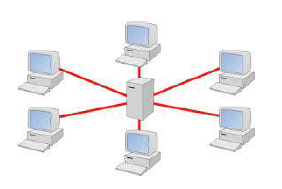
\includegraphics[width=3.0in]{2018spring/figures/20q_a.png}}
\caption{Star Topology}
\label{fig:20q_a}
\end{figure}

\item[21.] Consider a data link layer with the following parameters: Frame transmission time at the sender is $\mathrm{t}_\mathrm{f}=20$ microseconds. ACK or NAK transmission time at the receiver is $\mathrm{t}_\mathrm{ack} = 10$ microseconds. Link propagation delay on both directions is $\mathrm{t}_{\mathrm{prop}} = 25$ microseconds. Suppose frame processing time at both sender and receiver is negligible, i.e., $\mathrm{t}_{\mathrm{prop}] = 0$. Finally, overall round-trip probability of frame error on the link is $r=0.04$. 

    \begin{enumerate}
        \item Assume that for the Stop-and-wait ARQ scheme, the TIMEOUT at the sender is chosen optimally. What is the resulting throughput (frames/second)?
        \item  In the Go-Back-N ARQ scheme, if the link is error free, what is the minimum window size $N$ that is able to keep the link busy?
        \item Choose window size in Part b and now consider the link error probability $r=0.04$. What the throughput (frames/second) of the Go-Back-N ARQ scheme?
    \end{enumerate}

\end{enumerate}
\end{document}